\documentclass[12pt]{examnotes}

\header{ESC3701 Monetary Economics III}
%%%%%%%%%%%%%%%%%%%%%%%%%%%%%%%%%%%%%%%
\begin{document}

\obeylines  
\setlength\baselineskip{15pt}

\h{Part 1}
\sh{Chapter 1: Why study money, banking and financial markets.}
\ra A security or financial instrument is a claim on the issuer’s future income or assets (which is any financial claim or piece of property that is subject to ownership). 
\ra A bond is a debt security that promises to make payments periodically for a specified period of time. 
\ra An interest rate is the cost of borrowing or the price paid for the rental of funds. 
\ra Financial Crises is a  major disruption in the financial markets characterised by a sharp decline in asset prices and the failure of many financial and non-financial firms. 
\ra GDP (aggregate output) is the market value of all final goods and services produced in a country during the course of the year, which excludes purchase of goods that have been produced in the past and excludes purchase of stocks or bonds. Intermediate goods are not counted.
\ra Aggregate income is the total income of factors of production from producing goods and services per country per year. {\bf GDP = Aggregate Income.} 
\ra When GDP is calculate with current prices it is called nominal GDP. 
\ra GDP measured with constant prices is referred to as real GDP. Therefore values only change if actual production changed.
\ra 3 Aggregate price levels, expressed as price index against base year 100.
\vspace{6pt}
\rn{1} GDP deflator =  $\displaystyle\frac{\text{nominal GDP}}{\text{real GDP}}$ 
\vspace{6pt}
\rn{2} PCE deflator =  $\displaystyle\frac{\text{nominal personal consumption expenditures}}{\text{real personal consumption expenditures}}$ 
\vspace{6pt}
\rn{3} Consumer Price Index measured by pricing a basket of goods and services brought by a typical urban household.
\ra To convert nominal to real divide by price index. Annualised basis is a basis converted to a year. 
\vspace{6pt}
\ssh{Meaning of a security and how it facilitates direct lending and borrowing}
\ra A security or financial instrument is a claim on the issuer's future income or assets. 
\ra To facilitate direct lending securities are sold in financial markets where the lender-savers channel funds to the borrower-spenders. 
\ra Common securities include bonds or stocks. 
\ra Securities are assets to the lender-savers and liabilities to the borrower-spenders. 
\ra Securities facilitate moving funds from people with an excess to the people who have profitable opportunities. 
\ra SA the major instrument of monetary policy is the control of an interest rate called the repo rate. \ra SARB – sets the repo rate.
\ra The repo rate in South Africa is the equivalent of the federal funds rate in the USA.
\ra The repo rate is a short-term interest rate which represents an interest rate paid by commercial banks to the SARB to obtain reserve funding (i.e. borrowing money from the SARB), yet it impacts on all interest rates in the economy. Thus changes in the repo rate impact the economy at large.

\ssh{Common stock, its purpose and how it affects business investment decisions.}
\ra A common stock represents a share of ownership in a company. 
\ra It is a security, and is a claim on the earnings and assets of the corporation. 
\ra Selling stock is way to raise funds for financing the companies activities.
\ra It affects business decisions as higher stocks prices in the stock market mean that the company will be able to raise more finance through selling stock at higher prices. 

\ssh{List two ways in which the quantity of money may affect the economy}
\rn{1} Through the aggregate price level 
\rn{2} Through interest rates. 

\ssh{Difference between nominal and real GDP and their uses}
\ra Nominal GDP is when the total value of final goods and services is calculated using current prices. \ra Real GDP is calculated with constant prices, given at a base year. 
\ra Nominal GDP can be misleading as an increase could be due to a rise in the price level or an actual increase in final good and services. 
\ra An increase in Real GDP can only be from an increase in final goods and services and not and increase in prices. 

%%%%%%%%%%%%%%%%%%%%%%%%%%%%%%%%%%%%%%%
\sh{Chapter 2: Overview of financial system}

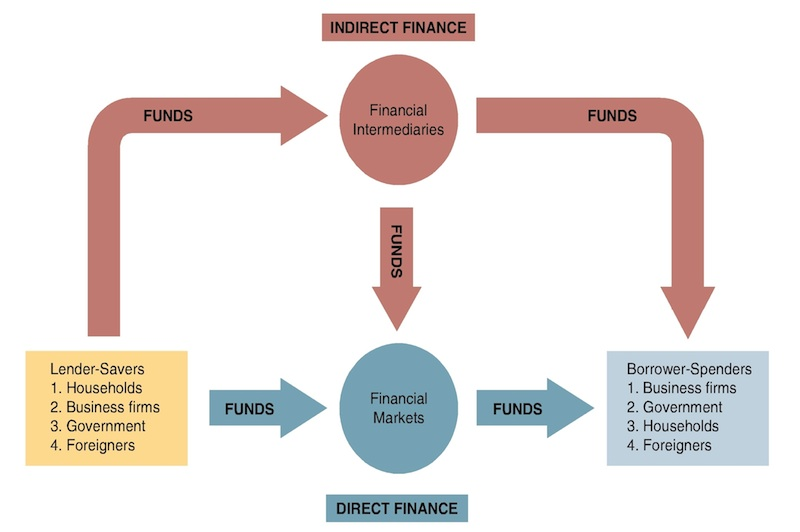
\includegraphics[scale=0.5]{./imgs/2finint.jpg}
\ra Direct finance: borrowers borrow funds directly from financial markets by selling securities
\ra Indirect finance: a financial intermediary borrows funds from lender-savers and then uses these funds to make loans to borrower-spenders.
\ra Financial markets are critical for producing an efficient allocation of capital which contributes to higher production and efficiency for the economy as a whole.
\ra Structure of financial markets
\rn{1} Debt and Equity Markets
\rna Short-term less than a year. 1-10 years are intermediate. $>10$ is long-term 
\rna Firms or individuals can obtain funds through issuing debt instruments (bonds/mortgage) or issue equities (stock)
\rna A disadvantage of equities is the holder is a residual claimant, the firm must pay debt holders first before its equity holders. 
\rna A advantage to holding equities is the direct benefit of increased firm profits versus the fixed amounts of debt, because of ownership rights of equities.
\ra Brokers are agents of investors who match buyers with sellers, dealers link buyers and sellers by buying and selling at stated prices. 
\rn{2} Primary and Secondary Markets
\rna Primary market for initial issues of securities (Investment banks). 
\rna Secondary markets (JSE) make securities more liquid, also set benchmark prices for the primary market. 
\rn{3} Exchange and OTC markets
\rna Secondary markets.
\rna Exchanges, central location where buyers and sellers of securities conduct trades
\rna OTC dealers  at different locations sell securities to anyone willing to pay their prices. Similarly competitive to exchanges due to technology.
\rn{4} Money and Capital Markets
\rna Money market: short-term securities
\rna Capital markets: 1 year or greater.1

\ssh{Financial market instruments}

\ra Money market short-term debt instruments.
\rn{1} US Treasury Bills. Short-term, no interest payments, set payment at maturity, sold at a discount. Most liquid and safest. Mainly held by banks.
\rn{2} Negotiable Bank Certificates of Deposit: a certificate of deposit (CD) is a debt instrument sold by a bank to depositors that pays annual interest of a given amount and at maturity pays back the original price. Negotiable CD’s are traded in secondary markets.  Big source of funds for banks.
\rn{3} Commercial Paper is a short-term debt instrument issued by large banks and well-know corporations.
\rn{4} Repurchase agreements are effectively short-term loans less than 2 weeks for which Treasury bills serve as collateral. Big source of funds for banks. Issued mainly by corporations.
\rn{5} Federal Funds, overnight loans between banks using their deposits at the Federal reserve.
\vspace{6pt}
\ra Capital Market for longer term debt.(Riskier than money market) 
\rn{1} Stocks. Largest security in capital market, Held by households and institutions.
\rn{2} Mortgages are loans to households or firms to purchase housing, land or real structures that serve as collateral. Largest debt market in US. 
\rna  Mortgage back security is a bond like instrument backed by a bundle of individual mortgages whose interest and principle payments are collectively paid to the holder-of the security.
\rn{3} Corporate Bonds. Issued by corporations with strong credit ratings. Convertible bonds can be changed into stock anytime up till maturity. Principle buyers are life insurance, pension funds households and other large holders. Not as liquid as government securities. Larger than new stock issues.
\rn{4} US Government Securities. Most liquid security.
\rn{5} US Government Agency Securities
\rn{6} State and Local Government Bonds (Municipal bonds). Issued by state and local governments for big projects, exempt for income tax. Banks largest holders.
\rn{7} Consumer and Bank Commercial Loans.

\ssh{Indirect finance and 4 financial intermediary functions}
\ra The basic function of financial markets is to channel funds from savers who have excess funds to spenders who have a shortage of funds. 
\ra Direct finance is when borrowers borrow funds directly from lenders by selling them securities
\ra The process of indirect finance using financial intermediaries is call financial intermediation.
\ra More important source of funds for corporations than securities markets.
\ra Financial intermediaries are financial institutions that acquire funds by issuing liabilities and, in turn use those funds to acquire assets by purchasing securities or making loans.
\ra Indirect finance involves an intermediary that stands between lenders and borrows and helps transfer funds from one to the other. 

\ssh{Transaction Costs / Liquidity services}
\ra Time and money spent in carrying out financial transactions.  
\ra Intermediaries can reduce transaction because they benefit from economies of scale due to expertise and size. 
\ra Intermediaries provide liquidity services that make it easier for customers to conduct transactions. e.g Checking accounts to pay bills.

\ssh{Risk sharing}
\ra They sell less risky investment and then use the funds to purchase more risky investments. 
\ra They earn profit on the difference between the returns on risky assets they bought and the payments made on assets they sold. Also called asset transformation. 
\ra They help individuals to diversify and thereby lower the amount of risk through low costs and assets pooling.

\ssh{Asymmetric information}
\ra One party does not know enough about the other party to make accurate decisions.
\ra Intermediaries are better equipped and can alleviate asymmetric information problems. 
\ra Two forms
\rn{1} Adverse selection
\rna Occurs before the transaction
\rna Potential borrowers who are the mostly like to produce an undesirable outcome are the ones who most actively seek out a loan and are thus most likely to be selected. 
\rna Results in fewer loans to all as lenders hesitate to lend at all.
\rn{2} Moral hazard
\rna Occurs after the transaction. 
\rna The risk that the borrower will engage in activities undesirable to the lender hence increase in chance of default. 
\rna Reduces loans for all due hesitation to lend.
\rna If there were no asymmetric information there could still be a moral hazard problem because the lender knows there might be a default and reducing such risk is too costly, therefore still a moral hazard.
\ra Intermediaries are better equipped to screen out bad risk (reduce adverse selection) and monitor borrowers (reduce moral hazard)

\ssh{Economies of scope} 
\ra Lowering the cost of information production for each service by applying one information resource to many different services.
\ra Credit risk evaluation on corporation for loan and then sale of the corporation's bonds to the public.
\ra Creates conflict of interest (moral hazard problem) due to offering multiple services, and by information being concealed or misleading.

\ssh{Type of financial intermediates}
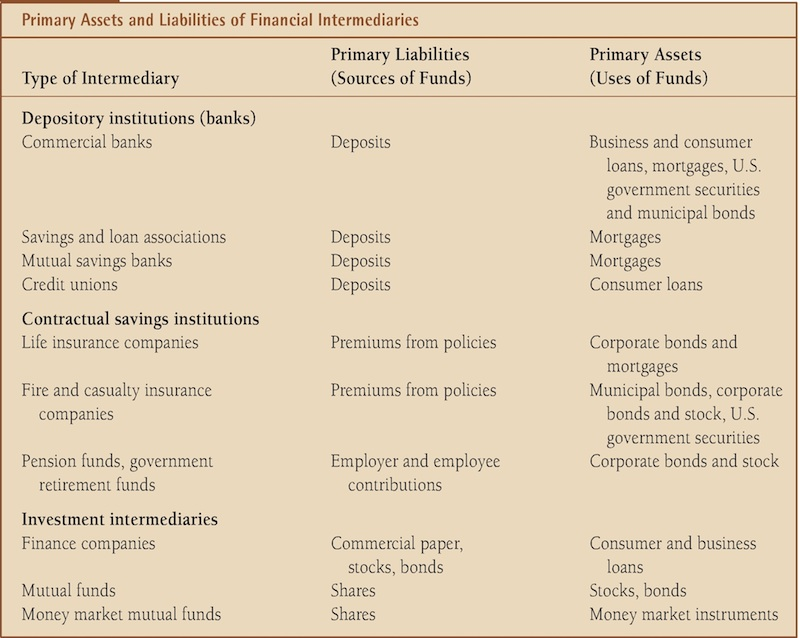
\includegraphics[scale=0.5]{./imgs/2types.jpg}
\ssh{Investment banks}
\ra Don't take deposits. 
\ra Advises corporations on type of security to issue and then purchase the security at a predetermined price and resells on the market (underwriting). 
\ra Act as deal makers and earn fees on mergers and acquisitions.

\ssh{Regulation of the financial system}
\ra To reduce asymmetric information problems
\rn{1} Increase information available to investors 
\rna Provisions of information is improved by requiring companies issuing securities to report details about assets and liability, earnings, sales of stock 
\rna Preventing insider trading. 
\rn{2} Ensure the soundness of the financial system. 
\rna Soundness is ensured by restrictions on entry, disclosure, restrictions on assets and activities, deposit insurance, limits on competition and restrictions on interest rates.


%%%%%%%%%%%%%%%%%%%%%%%%%%%%%%%%%%%%%%%
\sh{Chapter 3}


\ssh{Meaning of money}
\ra Money is defined as anything that is generally accepted in payments for goods or services or in repayment of debts.
\ra It is measured as currency plus deposits. Money = Currency + Deposits
\ra Currency is paper money and coins
\ra Wealth is the total collection of pieces of property that serve to store value such as bonds, art, land, houses and cars.
\ra Income is the flow of earning per unit of time.
\ra Money is a stock variable. 

\ssh{Functions of money}
\rn{1} Medium of exchange
\rna Solves the double coincidence of wants (finding some one who has what you want at the same time  they want what you have), leads to high transaction costs.
\rna Money promote efficiency by eliminating time spent exchanging goods and services
\rna Encourages specialisation and division of labour.
\rna Money reduces transaction costs.

\rn{2} Unit of account 
\rna It is used to measure value in the economy
\rna Lowers transaction costs by reducing the number of prices that need to be considered.

\rn{3} Store of value
\rna A repository of purchasing power over time.
\rna Money is the most liquid asset of all because it is a medium of exchange as it does not need to be converted to anything else.
\rna Not the most attractive store value and depends on the price level.
\rna During inflation less money is held.

\vspace{6pt}
\ra For a commodity to function as money it must be:
\rn{1} Easily standardised to ascertain value.
\rn{2} Widely accepted
\rn{3} It must be divisible
\rn{4} Easy to carry
\rn{5} Not deteriorate quickly

\ssh{Evolutions of payment systems}
\rn{1} Commodity money
\rna Made up of precious metals such as gold and silver
\rna From ancient times to several hundred years ago
\rna Problem is the form of money is heavy and hard to transport
 
\rn{1} Fiat money
\rna Paper currency decreed by governments as legal tender but not convertible into coins or precious metals.
\rna Advantage is that it is lighter then coins or precious metal
\rna  Can on be accepted as medium of exchange if there is trust in authorities and extremely difficult to counterfeit.
\rna Easy to change currency due to the legal guarantee, e.g. Euro.
\rna Disadvantages is easily stolen, and expensive to transport in large amounts because of bulk.

\rn{1} Checks
\rna An instruction from your bank to transfer money from your account to another account when check is deposited.
\rna 
\rn{1} Electronic payment
\rna 
\rna 
\rn{1} E-money


\ra  In South Africa currency is all the paper money and coins in circulation less cash held in bank vaults. 
\ra Deposits are all domestic private non-bank deposits in banks. 
\ra Government bank deposits deposits are excluded. There are 4 levels of deposit inclusion being M1A, M1, M2 and M3.

\textbf{Briefly distinguish between money and income, and money and wealth}
Money as above, where as wealth is the total collection of pieces of property of store value, which includes money, bonds, common stock, art, land, furniture car and houses. Money is a stock variable and is measured at a specific time, while income is a flow variable and is measured over a portion of time.

\textbf{List and explain the three primary functions of money.}
One, medium of exchange, money is used to pay for goods and services and minimising the costs involved in transacting. Two, unit of account, it is used to measure value in the economy and reduce costs. Three, store of value, its a repository of purchasing power over time, an enables delayed purchases.

Commodity, fiat, checks, Electronic payments are online, e-money: debit cards and pre-loaded smart cards. 

\textbf{Explain the meaning and implications of the government "printing" money}
Government does not print money SARB does. 1) Printed money goes to Government bank account to replace old currency or issue cash, and only increase M when government pays for goods or services. 2) SARB buys government securities which are then used to pay. 1 and 2 can lead to hyperinflation if mismanaged because of MV=PY. Zimbabwe as case study.

%%%%%%%%%%%%%%%%%%%%%%%%%%%%%%%%%%%%%%%
\h{Part 2}
\sh{Chapter 4}

\sh{Measuring Interest Rates}

$\textrm{PV}=\displaystyle\frac{CF}{(1+i)^n}$ \quad

\textbf{Yield to maturity}(IRR), PV of all future payments. $\rm{LV} = \displaystyle\sum_{n=1}^{N} \frac{C_n}{(1+r)^{n}}$ 
\textbf{4 types of credit market instruments:} 
1) Simple loan such as many money market instruments. simple interest rate equals yield to maturity. Use NPV  
2) fixed-payment loan (fully amortised loan), same payment every month, includes interest and principal, such as mortgages. Use IRR 
3) Coupon bond, pays a fixed coupon payment every year until maturity when face/par value is repaid, such as us treasury bonds, corporate bonds. Use IRR, \emph{but remember the face value payment at maturity must also be discounted.}
4) Discount bond, (zero coupon bond) bought a a discount of it face-value and then repaid at face value at maturity, us treasury bills, savings bonds. 
Current bond prices and interest rates are negatively related. When the interest rate rises, the price of the bond falls and vice versa. The yield to  maturity is greater than the coupon rate when the bond price is below its face value. 
Perpetuity (consol) aka current yield: $i_c=\displaystyle\frac{C}{P_c}$ 

\sh{The distinction between interest rates and returns}
Rate of return: $R=\displaystyle \frac{C+P_{t+1}-P_t}{P_t}$
Rate of return is defined as the payments to the owner plus the change in value, expressed as a fraction of its purchase price.
The return on a bond will not necessarily equal the yield to maturity on that bond, due to price fluctuations giving higher or lower capital gains. Prices and returns for long-term bonds are more volatile than those of shorter term bonds. 
The only bond whose return equals the initial yield to maturity is one whose time to maturity is the same as the holding period.
A rise in interest rates is associated with a fall in bond prices, resulting in capital losses on bonds whose terms to maturity are longer than the holding period.
The more distant a bond's maturity, the lower the rate of return that occurs as a result of the increase in the in the interest rate. 

\textbf{Interest rate risk}: Prices and returns for long-term bonds are more volatile than those for shorter-term bonds due the sensitivity of longer term bonds to interest rate changes. Due in lager fact to the term to maturity being more than the holding period.

\sh{The distinction between real and nominal interest rates}
Real interest rate(ex ante real interest rate) $r=i-\pi^e$ 
When the real interest rate is low there are greater incentives to borrow and fewer incentives to lend. 
More accurate indicator of the tightness of credit market conditions. 
Indexed bonds: Interest and principal payments are adjusted for changes in the prices level. They are useful because to monetary policy makers because subtracting their interest rates from a nominal rate on a non-indexed bond they give insight into expected inflation.

\sh{Chapter 5}
\sh{Determinants of asset demand}
\textbf{Wealth}. An increase in wealth raises the quantity demanded of an asset, ceteris paribus. 
\textbf{Expected Return} An increase in an asset's expected return relative to that of an alternative asset raises the quantity demand, ceteris paribus. 
\textbf{Risk} If an asset's risk rises relative to that of alternative assets, its quantity demanded will fall, ceteris paribus. 
\textbf{Liquidity}. The more liquid an asset is relative to alternative assets, ceteris paribus, the more desirable it is, and the greater will be the quantity demanded. 
\textbf{Theory of Portfolio choice} How much of an asset people want to hold in their portfolios and is a summary of the above conditions. 

\sh{Supply and demand in the bond market}
\textbf{Demand curve}, relationship between quantity demanded and price or interest rate. It has a downward slope indicating lower prices for the bond the quantity demand is higher, ceteris paribus.
\textbf{Supply curve}, relationship between quantity supplied and price, ceteris paribus. Higher prices means higher supply.
\textbf{Market Equilibrium}.Clearing price. Quantity of bonds demanded equals quantity of bonds supplied. The market head towards this point and settles. $\rm{B^d}=\rm{B^s}$
\textbf{Excess supply}, people want to sell more bonds than others want to buy. \textbf{Excess demand}, people want to buy more bonds than others want to sell. 
Given diagram, the asset market approach, which are in terms of stocks of assets and not flows.
If households save more, wealth increases.

\begin{center}
  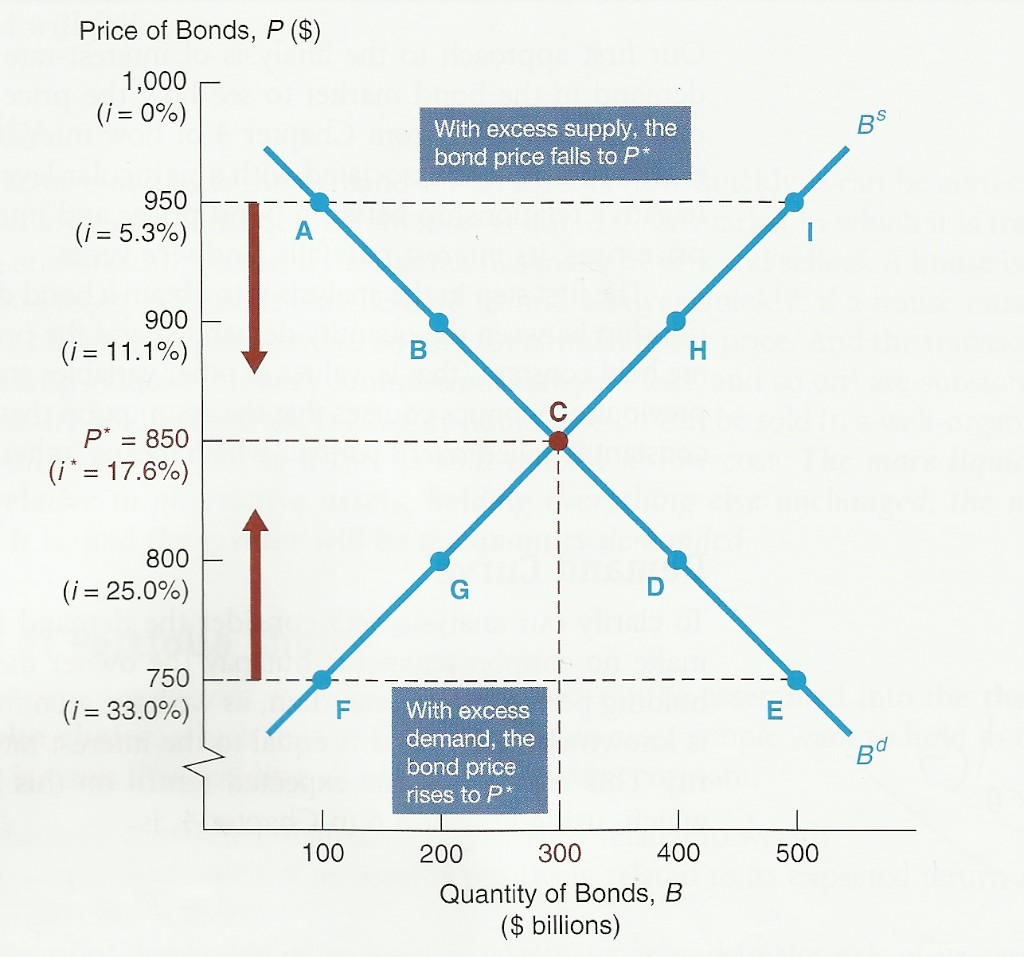
\includegraphics[scale=0.4]{./imgs/supplydemand.jpg}
\end{center}

\sh{Changes in Equilibrium interest rates}
\begin{center}
  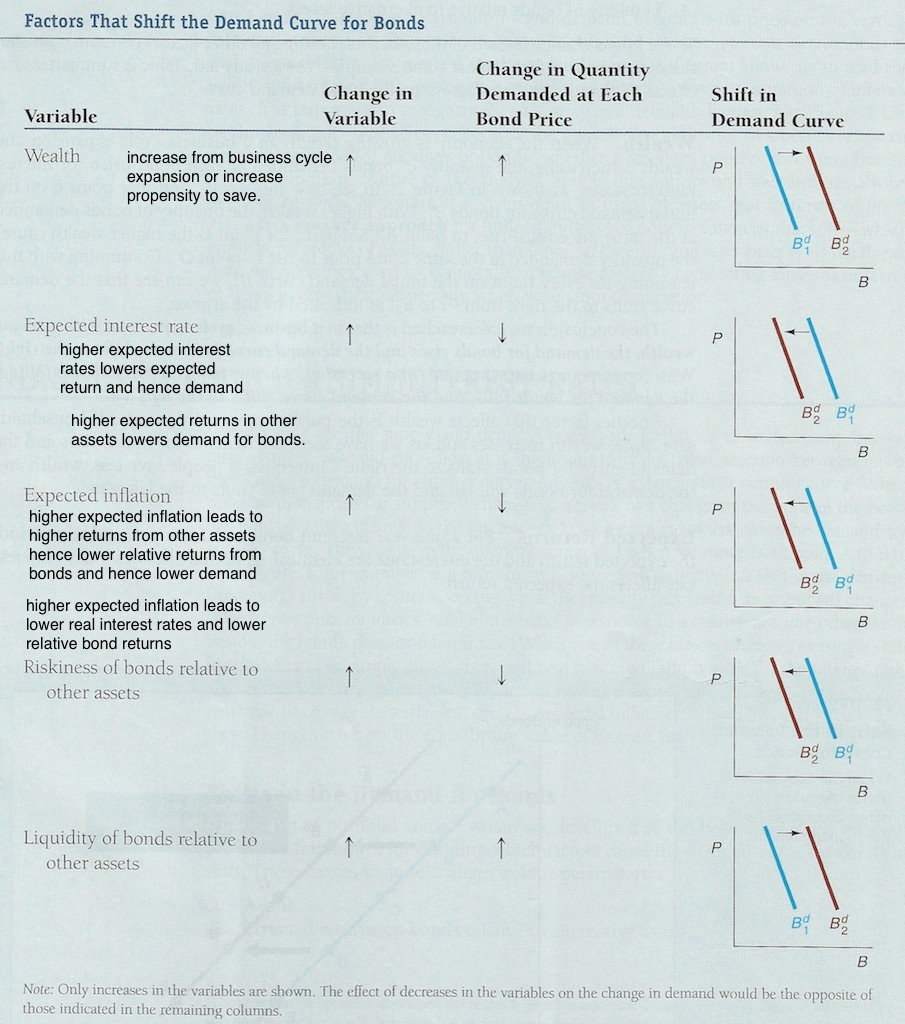
\includegraphics[scale=0.5]{./imgs/demandshift.jpg}
\end{center}
\begin{center}
  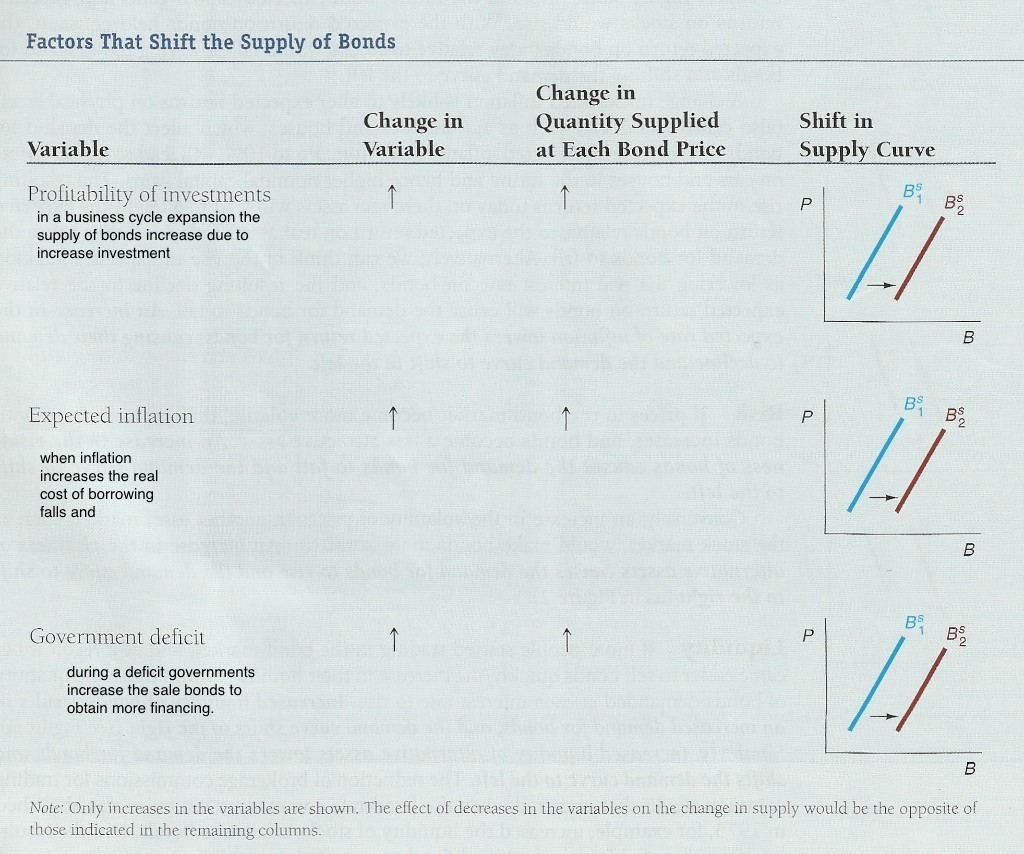
\includegraphics[scale=0.5]{./imgs/supplyshift.jpg}
\end{center}

\sh{Changes in the interest rate due to expected inflation, the Fisher Effect}
When expected inflation rises, interest rates will rise, also called the Fisher Effect. Ambiguous change in quantity, but certain increase in interest rate.
\begin{center}
  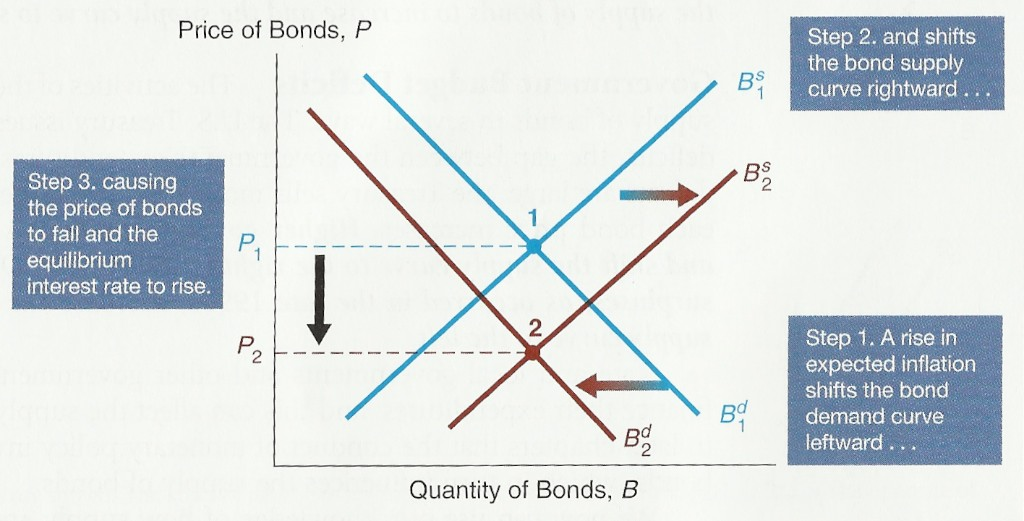
\includegraphics[scale=0.4]{./imgs/changeexpecteinflation.jpg}
\end{center}
\sh{Changes in the interest rate due to a business cycle expansion}
Amounts of goods and services rise with a corresponding increase in national income and business has more opportunities to expand, therefore they increase the supply of bonds, further the increase in wealth will, via the theory of portfolio choice, increase the demand for bonds. Ambiguous change in interest rate but certain increase in quantity.
\begin{center}
  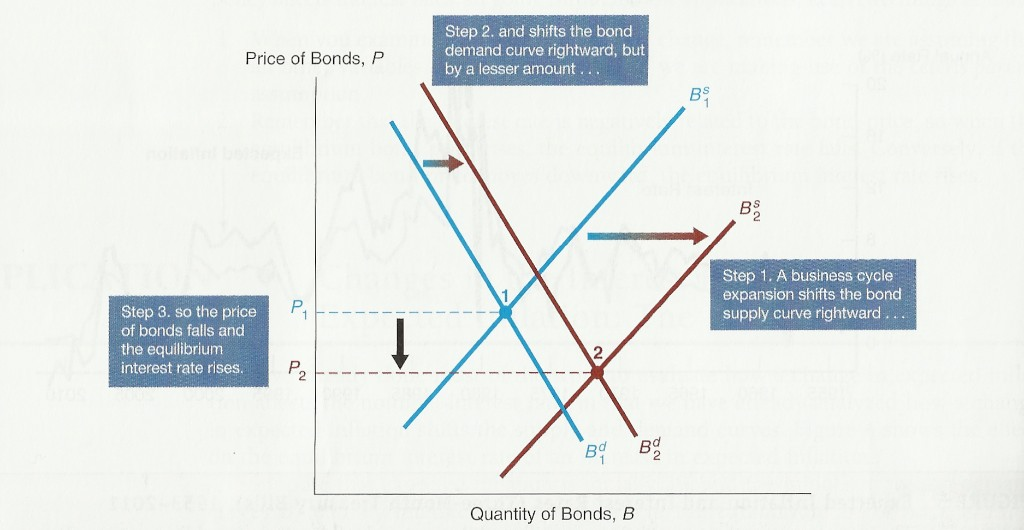
\includegraphics[scale=0.4]{./imgs/fig6.jpg}
\end{center}

\sh{Supply and demand in the market for money: The liquidity preference framework}
$\rm{B^S+M^S=B^d+M^s}$
Simplifying assumptions: Assumes there are only two kinds of assets, money and bonds and implicitly ignores any effects in interest rates from changes in expect returns on real assets such as cars. Assumes money as a zero rate of return as it earns no interest. Supply curve is vertical which is not the case in South Africa.
Demand curve: As the interest rate rises the expected return of money relative to bonds falls and the demand for bonds increases. The quantity of money demand and interest rate are negatively related because of the opportunity cost.
Supply curve: Central bank supplies a fixed quantity.
Equilibrium: $\rm{M^s=M^d}$ at the intersection of the supply and demand curves.
When the price level increase more money will be demanded to restore purchasing power.
\begin{center}
  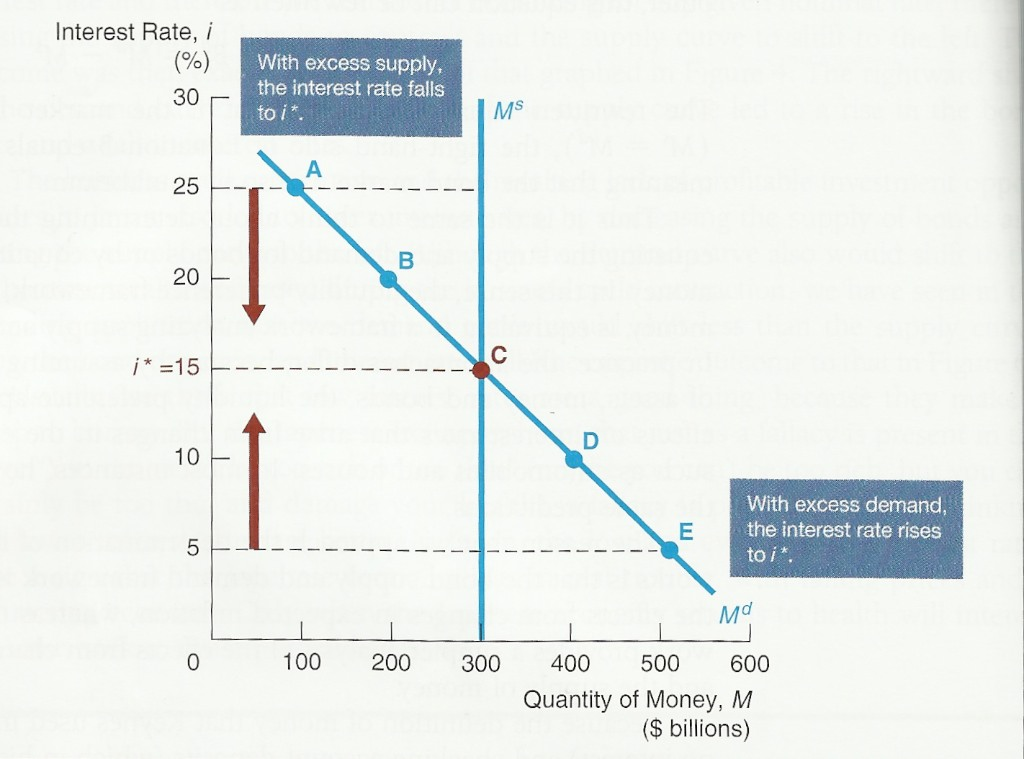
\includegraphics[scale=0.4]{./imgs/c5fig8}
  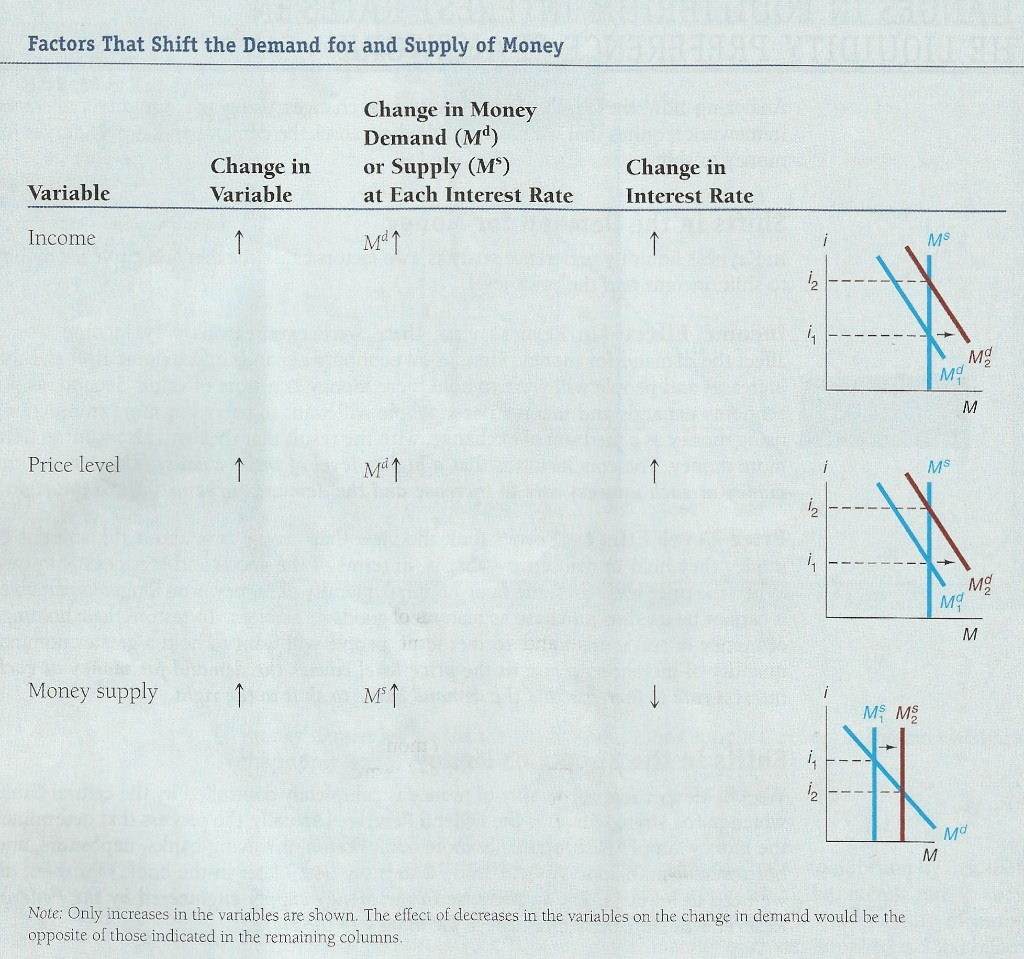
\includegraphics[scale=0.4]{./imgs/c5ft4.jpg}
\end{center}

1) The income effect of an increase in the money supply is a rise in interest rate in response to the higher level of income.
2) the price-level effect from and increase in the money supply is a rise in interest rates in response to the rise in price level.
3) the expected-inflation effect of an increase in money supply is a rise in interest rates in response to the rise in the expected inflation rate.

\begin{center}
  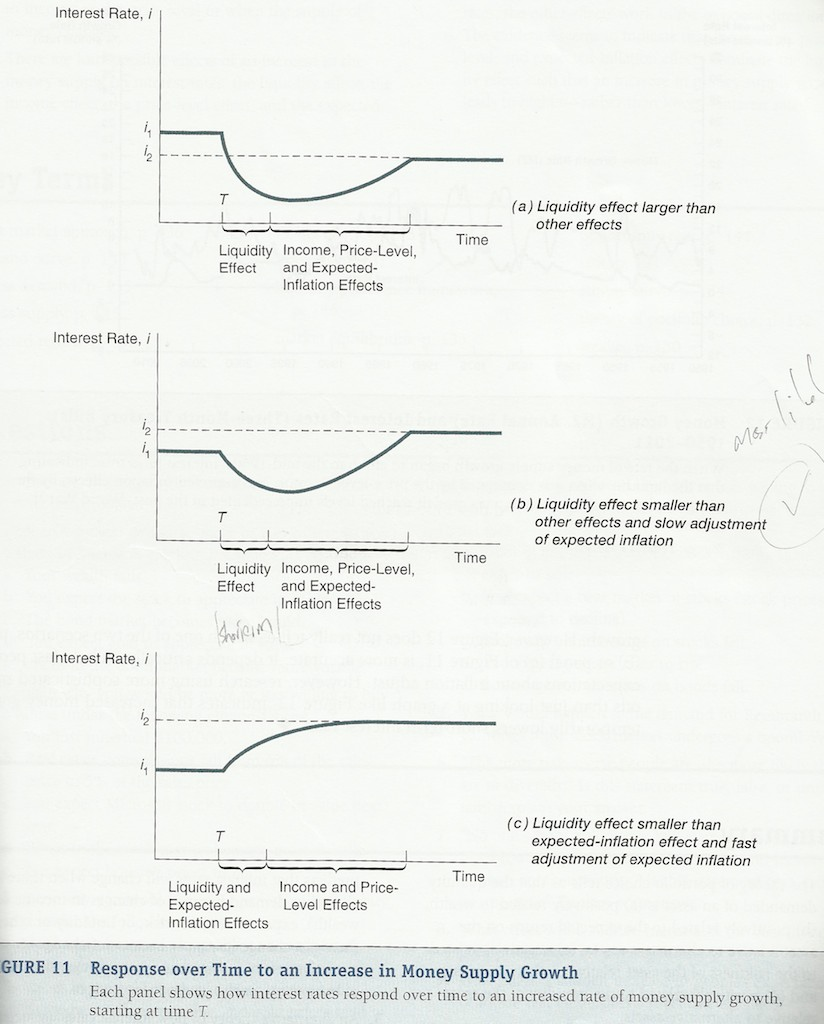
\includegraphics[scale=0.5]{./imgs/c5f11.jpg}
\end{center}
\colorbox{red}{\textcolor{white}{page 153 for quick review.}}

%%%%%%%%%%%%%%%%%%%%%%%%%%%%%%%%%%%%%%%
\sh{Chapter 6}


\textbf{Questions}
\textbf{Explain the meaning of the risk structure of interest rates. List and explain the three factors which affect the risk structure of interest rates using a supply of/demand for bonds-framework.}
The risk structure of interest rate is the relationship among interest rates on bonds with the same maturity.
3 Factors affecting risk structure 1) Default risk. Default risk is the risk of the issuer of the bond being unable or unwilling to make interest payments or pay off the face value when the bond matures.  Bonds are such as US Treasury bonds are considered default free, as they are backed by the US government which can increase taxes or print money to meet it obligations. The risk premium is the difference between bonds with default risk and bonds that are default free. A bond with default risk will always have a positive risk premium and an increase in its default risk will raise the risk premium. Credit ratings agencies provide information about the likelihood of a bond issuer defaulting. 
2) Liquidity, the higher the bond's liquidity the more appealing it is and therefore there would be a rightward shift in the demand for bonds curve the more liquid bond. US Treasury bonds are the most liquid of all bonds. (use graph below to show increased spread due to liquidity) 3) Income tax considerations. Bonds that are exempt from tax have higher expected returns and hence there is an increased demand for them. (use graph below to show)
\begin{center}
  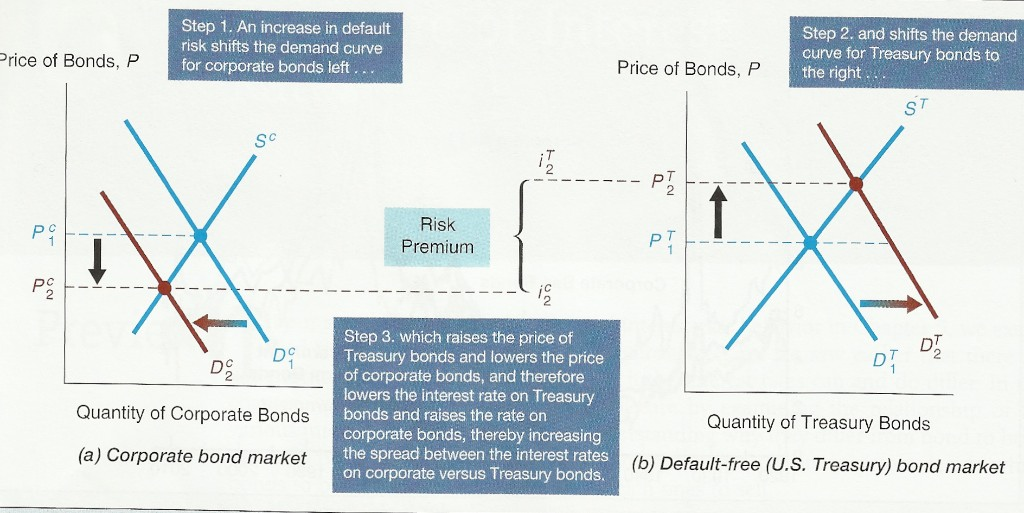
\includegraphics[scale=0.45]{./imgs/c6f2.jpg}
  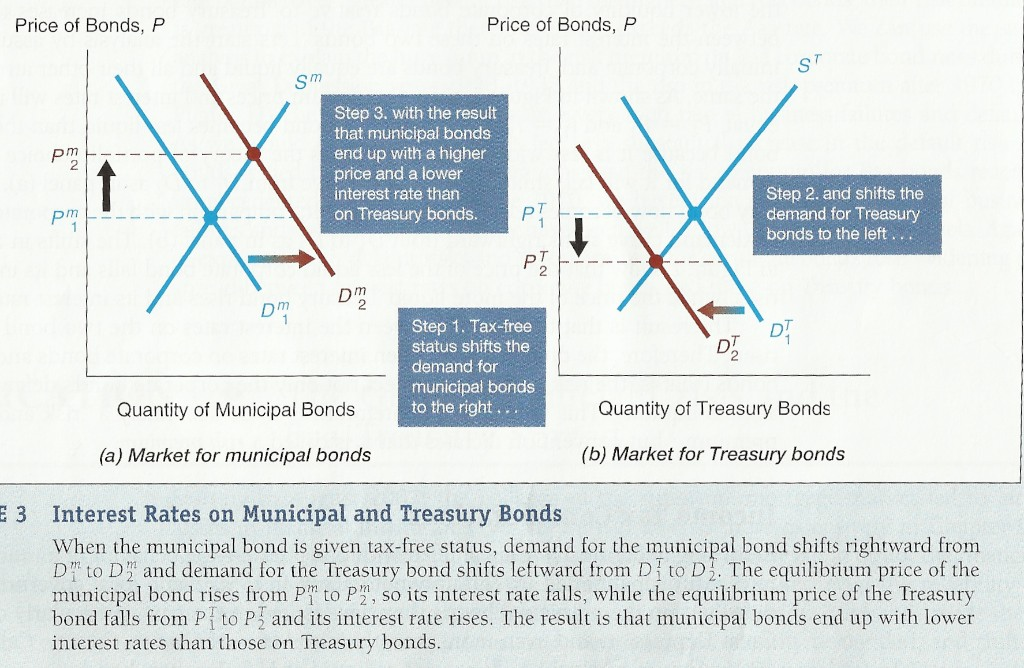
\includegraphics[scale=0.4]{./imgs/c6f3.jpg}
\end{center}

\textbf{Explain the meaning of the term structure of interest rates and the yield curve. Draw a normal yield curve and explain why its shape applies. List three empirical observations of the yield curve.}
Bonds with identical risk, liquidity and tax characteristics may have different interest rates because their time remaining to maturity is different. A plot of the yield is called a yield curve. Yield curves can slope up, flat or downward (inverted). Upward sloping yield curves indicate long-term interest rates are higher than short term interest rates. 3 empirical observations are that 1) interest rates on bonds of different maturities move together over time, 2) when short-term interest rates are low, yield curves are more likely to have an upward slope and vice-versa 3) yield curves almost always slope upward. 
\begin{center}
  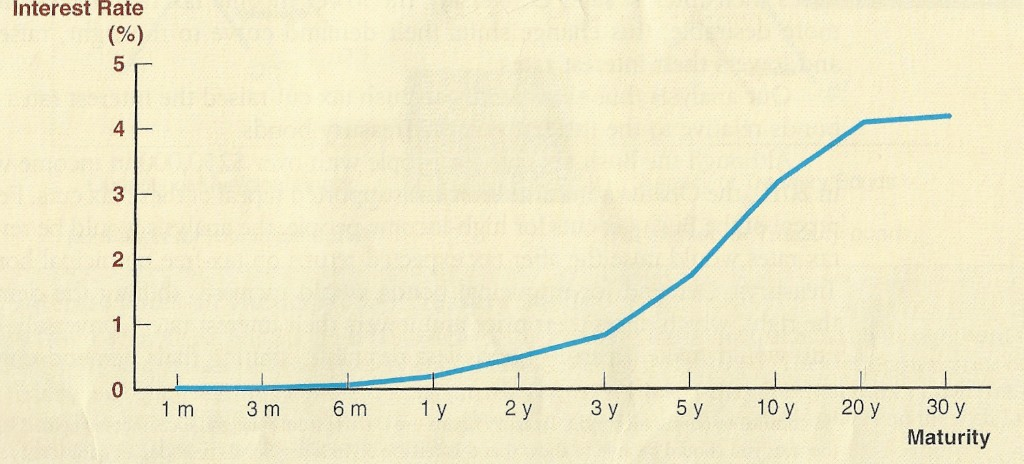
\includegraphics[scale=0.4]{./imgs/yieldcurve.jpg}
\end{center}

\textbf{Explain the assumptions and predictions of the expectations theory and how well it explains the three empirical observations of the yield curve.}
The interest rate on a long term-term bond will equal an average of the short-term interest rates that people expect to occur over the life of the long-term bond. The key assumption is that buyers of bonds do not prefer bonds of one maturity over another, so they will not hold any quantity of a bond if its expected return is less that that of another bond with a different maturity, i.e. perfect substitutes (same expected return). When the yield curve is upward sloping short term interest rates are expected to rise. When the yield curve is inverted the average of future short-term interest rates is expected to be lower than the current short-term rate, implying that short-term interest rates are expected to fall. If the yield curve is flat short-term interest rates are not expected to change. Fact 1) A rise in short term rates will raise people's expectation of future short-term rates and given that long-term rates are an average of short-terms rate they to will rise and hence move together. Fact 2) When short term rates are low people will expect them to rise and the average of future short-term rates rate is high relative to the current short-term rate hence upwards sloping and conversely for the inverted yield curve. Fact 3) It cannot explain this fact as it predicts a typical curve would be flat. 

\textbf{Explain the assumptions and predictions of the the segmented market theory and how well it explains the three empirical observations of the yield curve.}
Sees markets for different-maturity bonds as completely separate and segmented. The interest rate for each bond with a different maturity is then determined by supply and demand for that bond with no effect from expected returns. Bond are not substitutes at all due to the fact that investors have a strong preference for bonds of one maturity but not for another and are only concerned with the expected returns of their preference. This is due to the preference for a certain holding period. It explains fact 3) as the demand for short-term bonds is higher due to the lower risk hence higher prices and lower interest rates and similarly with long term bonds. This explain the normal upward slope. This theory is unable to explain fact 1) and 2), due to the fact that different maturity bonds having no influence on each others interest rates, and it is not clear how demand and supply for short-term bonds changes with the level of short term interest rates. 

\textbf{Explain the assumptions and predictions of the liquidity premium theory of the term structure and the preferred habitat theories of the term structure and how well they explain the three empirical observations of the yield curve.}
The liquidity premium theory states the the interest rate on a long-term bond will equal an average of short-term interest rates expected to occur over the life of the long-term bond plus a liquidity premium (term premium) that responds to supply and demand. Key assumption is that bonds of different matures are substitutes with their expected returns influencing one another, they are not perfect substitutes.
\colorbox{red}{\textcolor{white}{read summary page 175}}
\begin{center}
  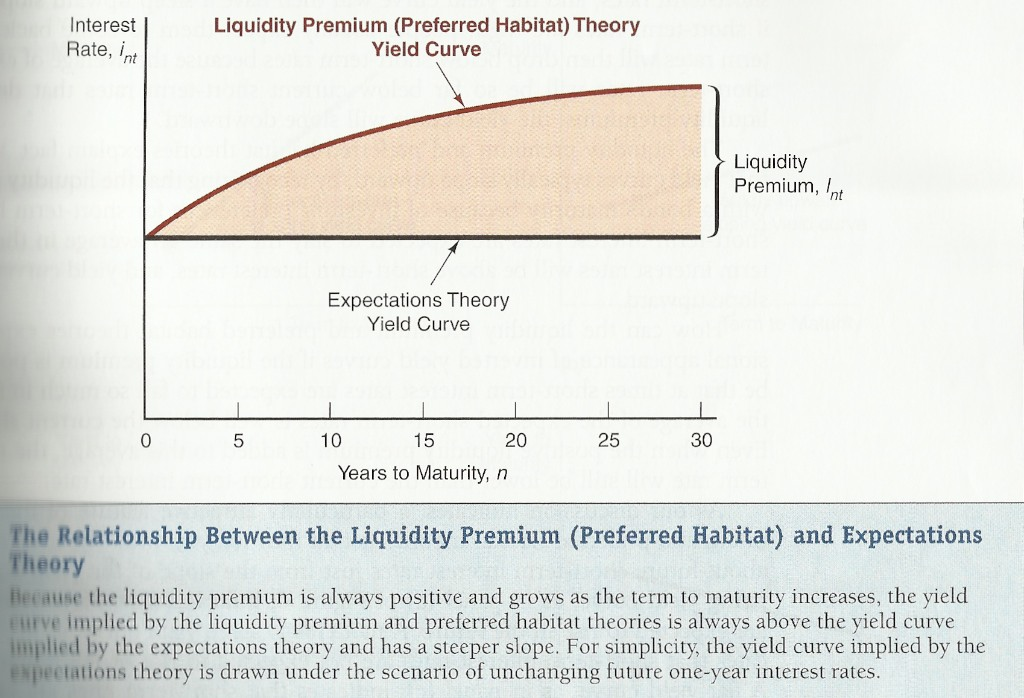
\includegraphics[scale=0.5]{./imgs/c6f5.jpg}
\end{center}



%%%%%%%%%%%%%%%%%%%%%%%%%%%%%%%%%%%%%%%
\h{Part 3}
\sh{Chapter 8}
\begin{center}
  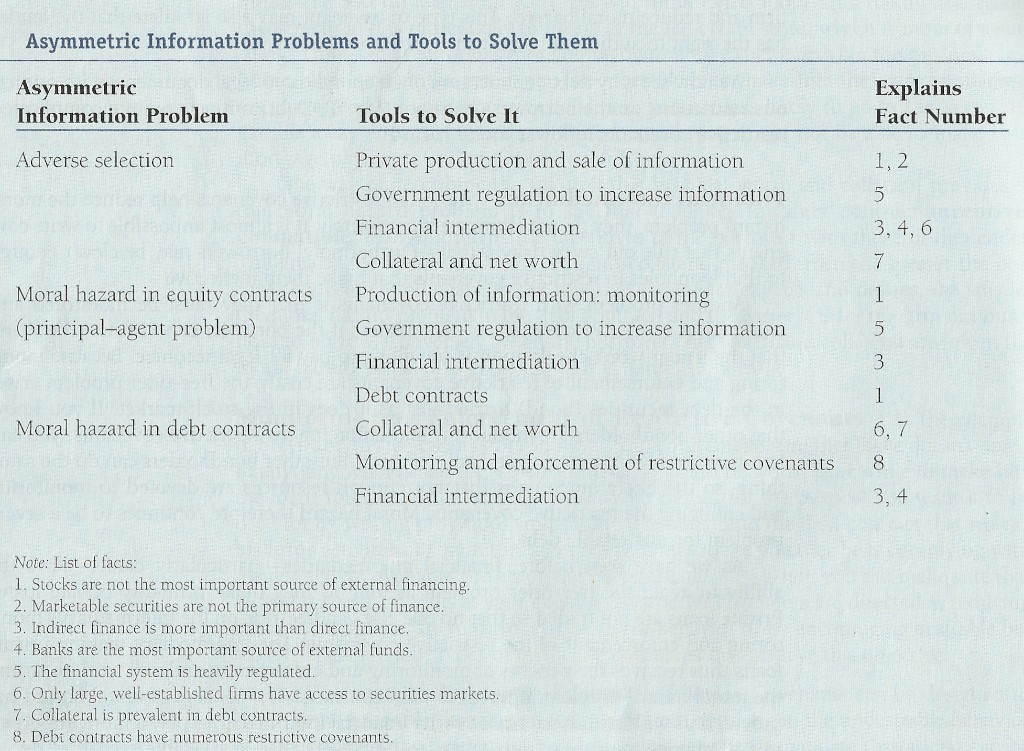
\includegraphics[scale=0.5]{./imgs/part3table.jpg}
\end{center}


\textbf{Questions}

\textbf{List eight basic facts about financial structure throughout the world}
1) Stocks are not the most important source of external financing for business
2) Issuing marketable debt and equity securities is not the primary way in which businesses finance their operations.
3) Indirect finance is more important than direct finance
4) Banks are the most important source of indirect finance
5) The financial system is heavily regulated
6) Only large well-established companies have easy access to securities markets
7) Collateral is a prevalent feature of debt contracts
8) Debt contract are complicated legal documents placing substantial restrictions on borrowers 

\textbf{Explain the role of financial intermediaries by referring to the problem of high transaction costs in financial transactions and the role of financial expertise}
Financial intermediaries stand between lender-savers and borrow-spenders. They enable funds to be transferred from people with non-productive opportunities to people with productive opportunities. In financial markets the costs of transacting is high. Financial intermediaries reduce transaction costs by taking advantage of economies of scales. They bundle funds together like mutual funds. The costs of a small transaction is similar to the cost of a large transaction. They increase diversification of risk, buy purchasing a range of securities, as small investors would be compelled to keep all their eggs in the same basket, to keep costs down. They have developed better expertise, such as computer technology, help desks and liquidity services (more transactions or being able to pay bills).

\textbf{Explain why marketable securities (debt and equity) are not the primary source of financing for businesses and how financial intermediaries and government regulation can partly overcome the problem of asymmetric information (adverse selection).}
The presence of the lemons problems keeps markets from being effective. Buyers will only buy if compensated for average default risk, knowledgeable buyers will realise they would be paying to much and therefore not buy. Only bad firms would buy at the lower average than what should be charged for their riskier investments, but investors would not want to sell therefore efficiency is reduced.
Lemons problems is a adverse selection problem, i.e. more high risk borrowers and fewer low risk borrowers leads to less lending overall. Asymmetric information problem.

Government regulations can reduce adverse selection buy forcing audit and reporting of internal financial details. Government cannot produce ratings as this would be politically difficult. Government regulations can go only so far because companies would always have more information than investors and bad firms make themselves look good.

Financial intermediaries are experts at producing information about firms and can get be returns hence produce more information, they overcome the free-rider problem by primarily making private non-traded loans so other investors cannot bid up prices.

\textbf{Explain, in general, why indirect financing is more important than direct financing and, in particular, why banks are the most important source of external finance for financing businesses. Then comment on the two statements: "The role of banks in lending will probably decline in future" and "The more established a firm is, the more likely it will issue securities to raise funds".}
Banks hold large portions of non-traded loans and not subject to free-rider therefore collect more info. Adverse selection is reduced by banks. Also banks have a collective reputation like car dealers. 
A better know company has more information available thereby reducing asymmetric information and investor are more willing to investor hence easier access to stocks.
As information about firms becomes easier to obtain the roles of bank will decline, largely in part due to technology.

%%%%%%%%%%%%%%%%%%%%%%%%%%%%%%%%%%%%%%%
\sh{Chapter 9}
\begin{center}
  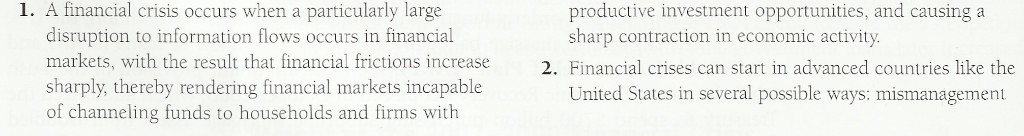
\includegraphics[scale=0.5]{./imgs/c9sum1.jpg}
    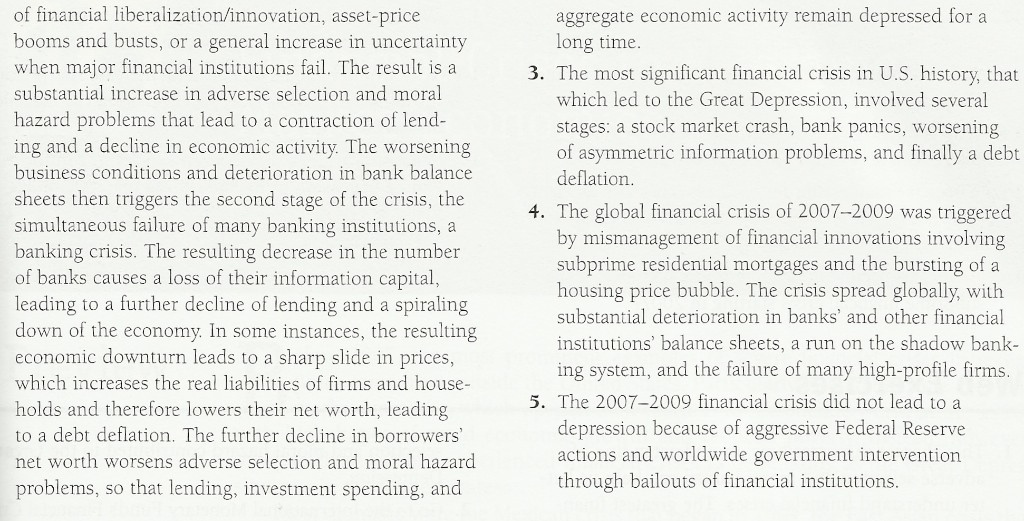
\includegraphics[scale=0.5]{./imgs/c9sum2.jpg}
\end{center}

%%%%%%%%%%%%%%%%%%%%%%%%%%%%%%%%%%%%%%%
\sh{Chapter 10}
\begin{center}
  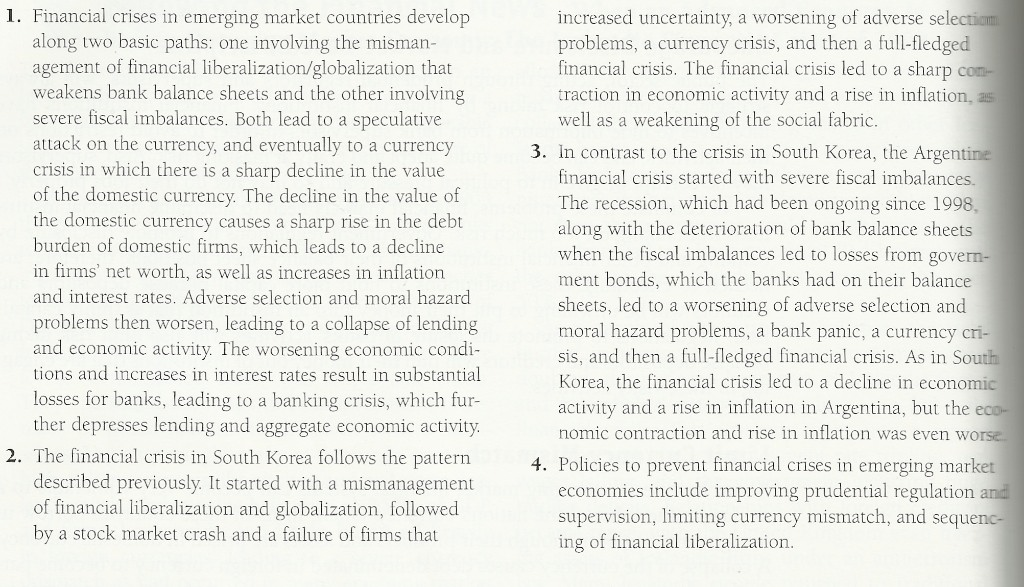
\includegraphics[scale=0.5]{./imgs/c10sum.jpg}
\end{center}

%%%%%%%%%%%%%%%%%%%%%%%%%%%%%%%%%%%%%%%
\sh{Chapter 11}
\begin{center}
  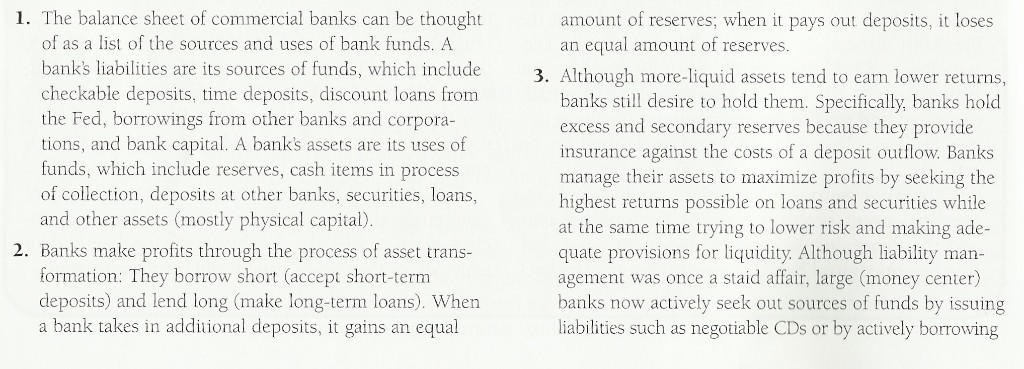
\includegraphics[scale=0.45]{./imgs/c11sum1.jpg}
  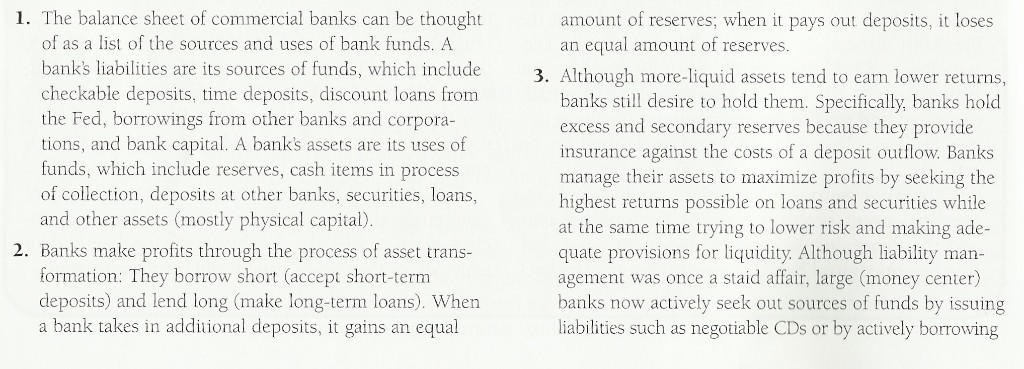
\includegraphics[scale=0.45]{./imgs/c11sum1.jpg}
\end{center}


%%%%%%%%%%%%%%%%%%%%%%%%%%%%%%%%%%%%%%%
\h{Part 4}
\sh{Chapter 14}
Central Bank Independence:
\textbf{FOR}: Political pressures would impart an inflationary bias due to their short-term focus on winning the next election; this could lead to a political business cycle, with expansionary policy just before an election and contraction policy after. It could also be used to fund budget deficits. Politicians also lack the ability to control monetary policy, and suffer larger affects of the agency problem. Empirical evidence suggest Independence is best for targeting inflation but central banks should be accountable to parliament.

\textbf{AGAINST}: 
Undemocratic to be controlled by a few elites, with a lack of accountability. There needs to be a coordinated effort between fiscal and monetary policy. Central banks may pursue narrow self interests and can be bureaucratic. 

\sh{Chapter 15}
\begin{center}
  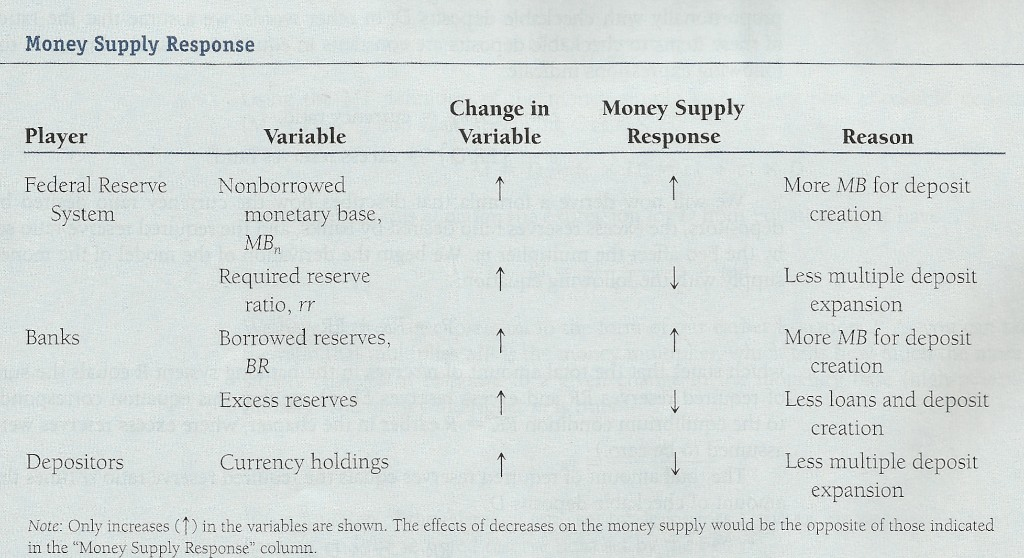
\includegraphics[scale=0.5]{./imgs/moneysupplytable.jpg}
\end{center}

\sh{Chapter 16}
\begin{center}
  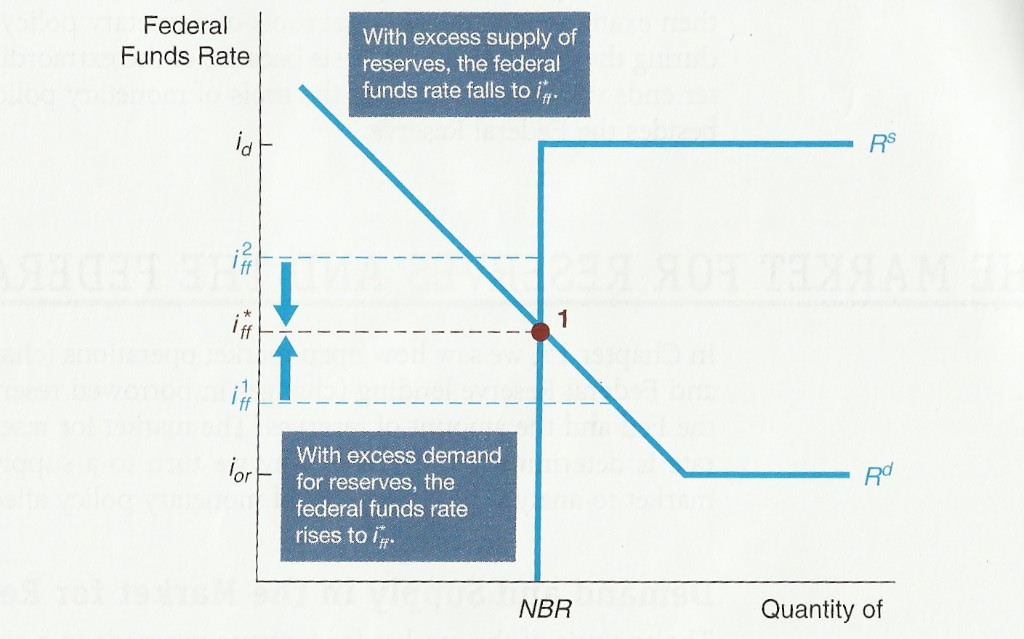
\includegraphics[scale=0.4]{./imgs/chapter6fig1.jpg}
  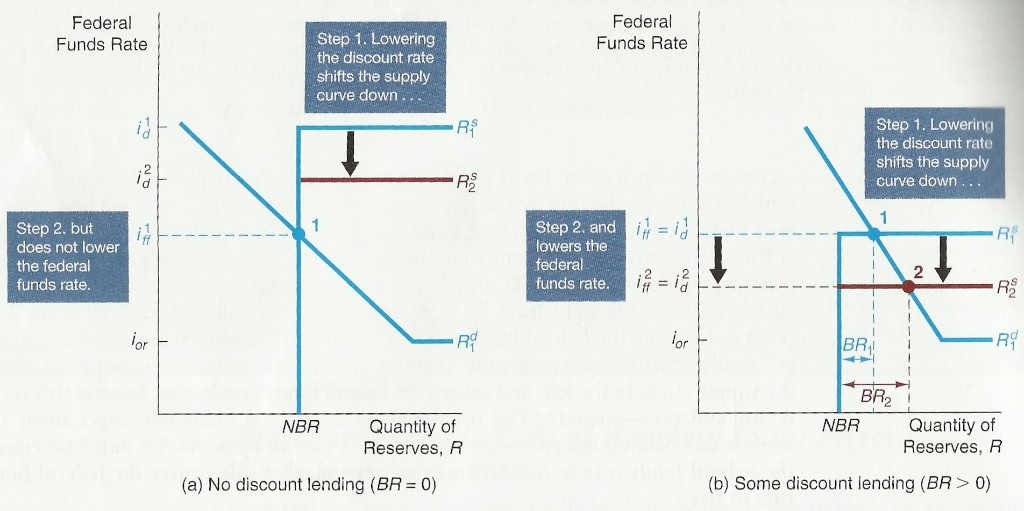
\includegraphics[scale=0.5]{./imgs/chapter16fig3.jpg}
\end{center}

\sh{Chapter 17}
\begin{center}
  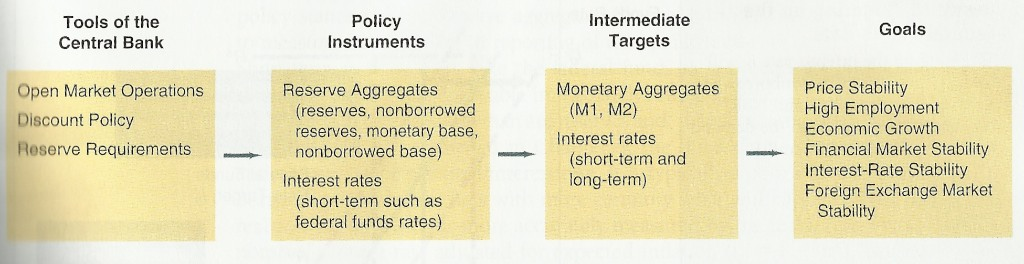
\includegraphics[scale=0.5]{./imgs/chap17fig2.jpg}
  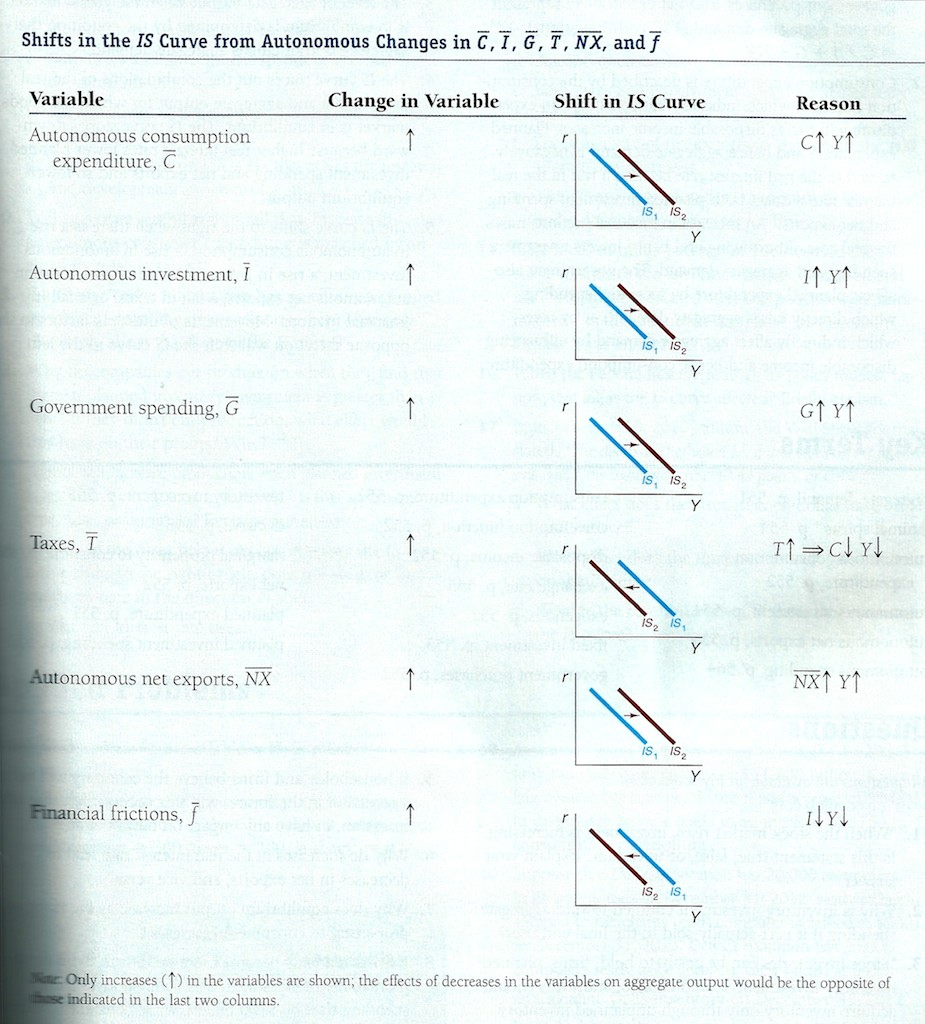
\includegraphics[scale=0.5]{./imgs/c21t1.jpg}
\end{center}


%%%%%%%%%%%%%%%%%%%%%%%%%%%%%%%%%%%%%%%
\h{Part 6}

\sh{Chapter 20}
Velocity of Money = $\displaystyle\frac{P \times Y}{M}$ 
Equation of Exchange: $M\times V=P \times Y$
\begin{center}
  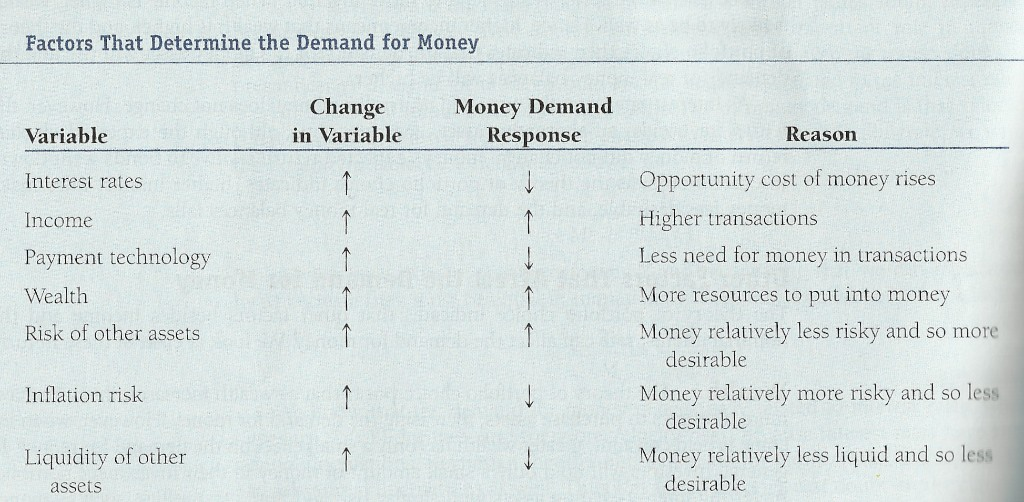
\includegraphics[scale=0.5]{./imgs/c20t1.jpg}
\end{center}

\sh{Chapter 21}
\begin{center}
  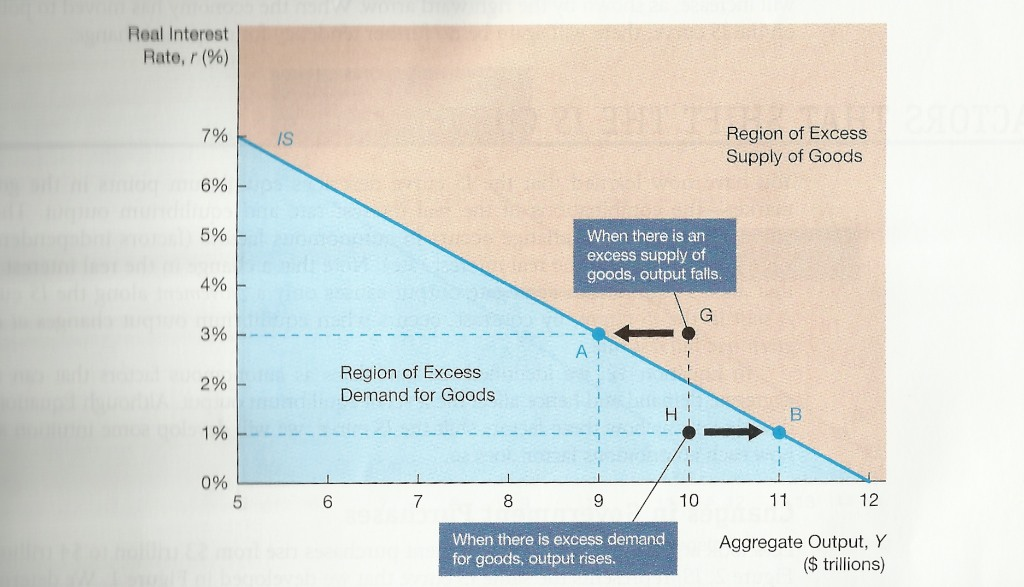
\includegraphics[scale=0.5]{./imgs/c21f1.jpg}
\end{center}

\sh{Chapter 24}
\begin{center}
  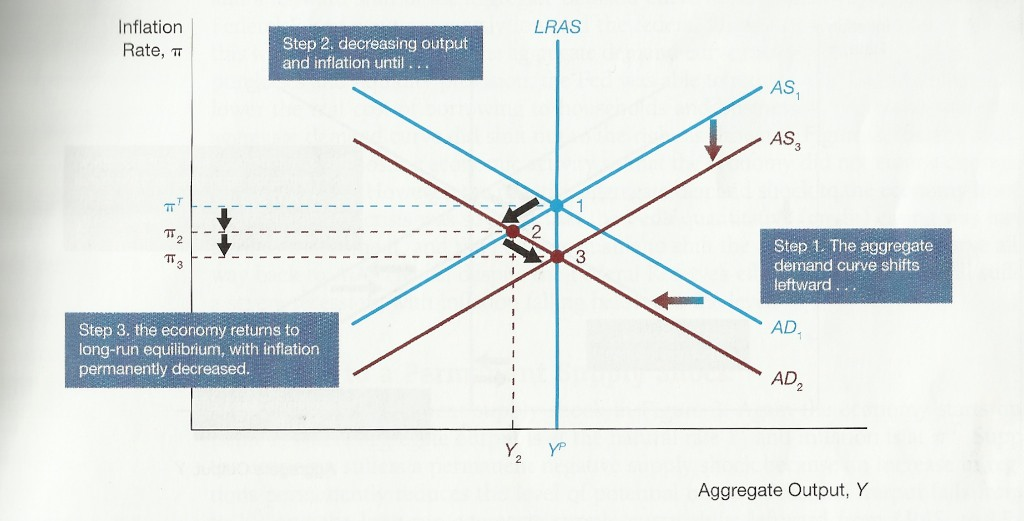
\includegraphics[scale=0.5]{./imgs/c24f1.jpg}
  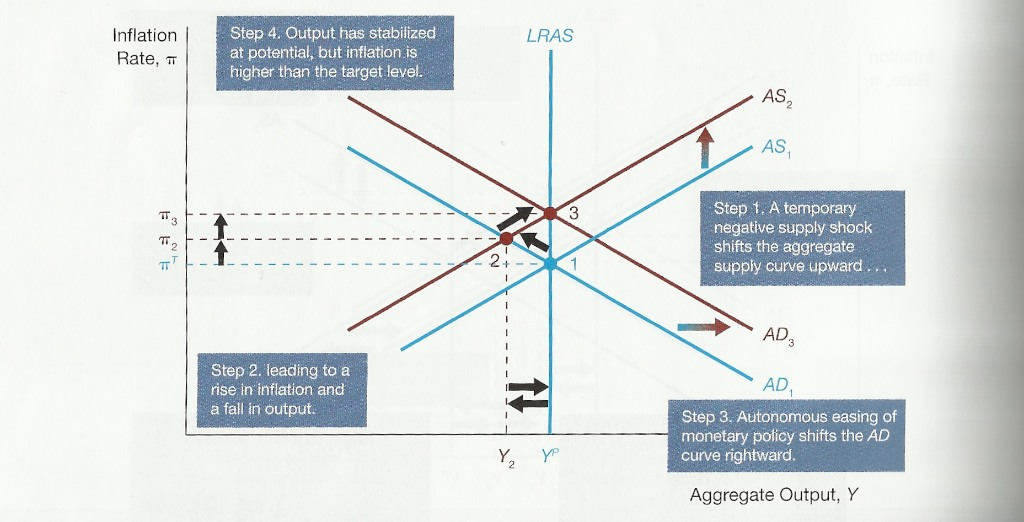
\includegraphics[scale=0.5]{./imgs/c24f7.jpg}
  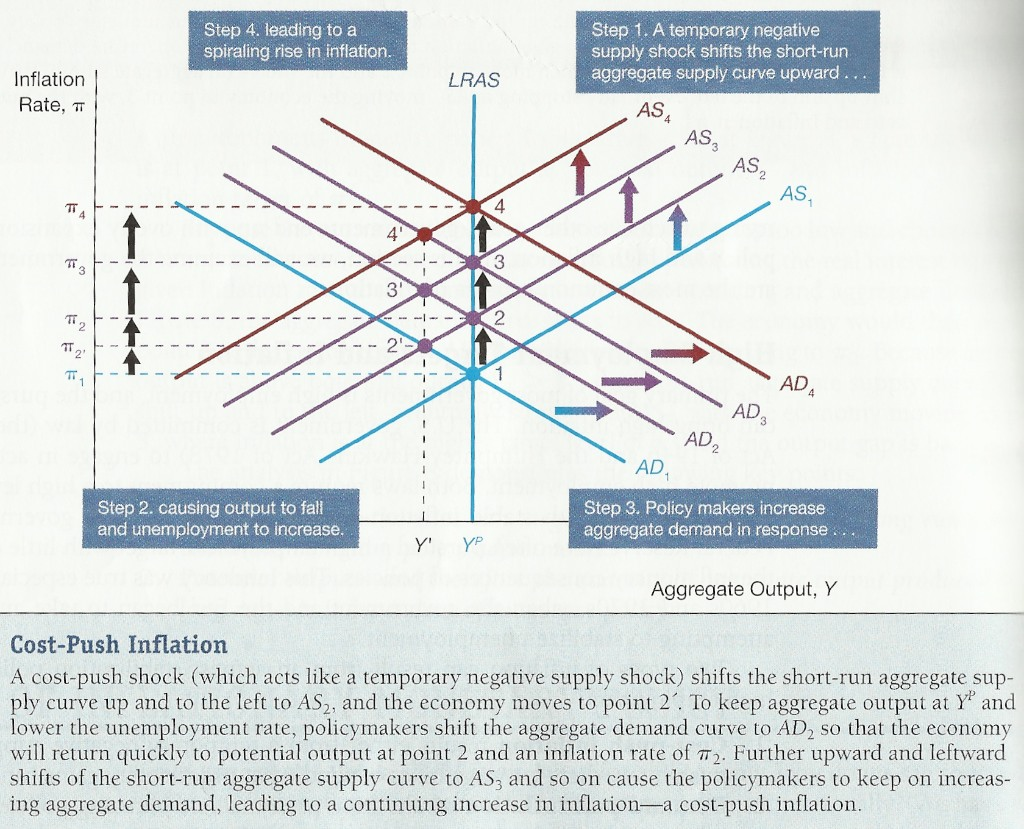
\includegraphics[scale=0.4]{./imgs/c24f9.jpg}
    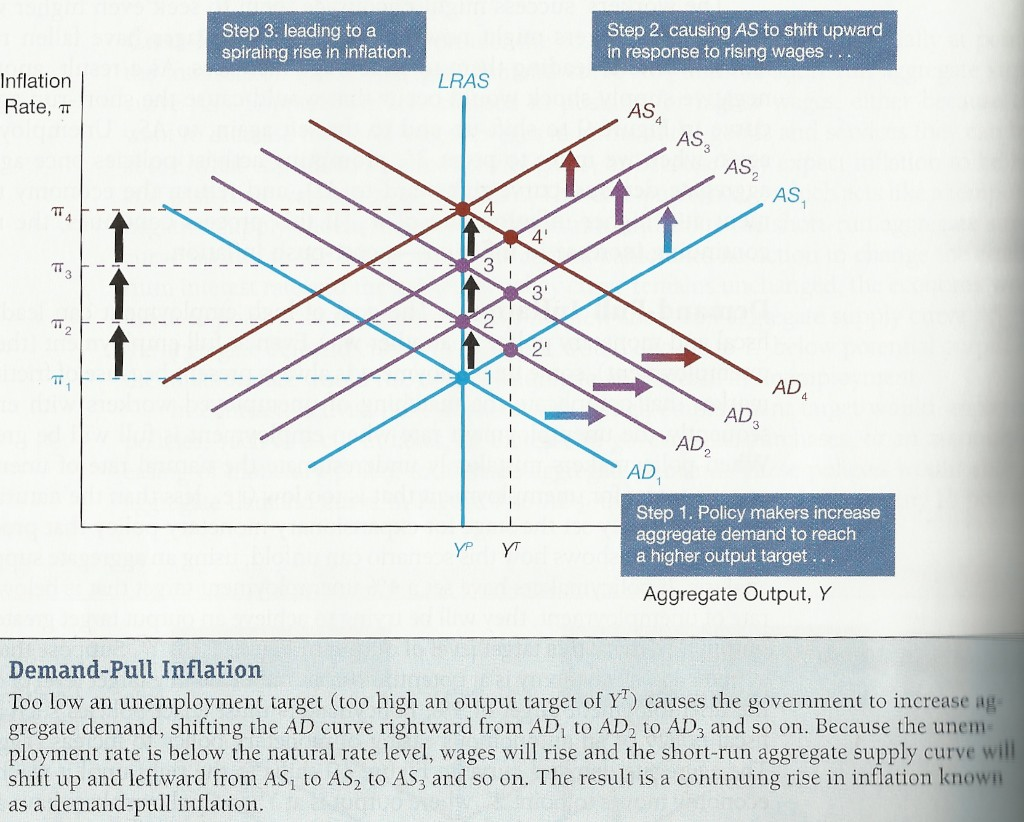
\includegraphics[scale=0.4]{./imgs/c24f10.jpg}
\end{center}
\colorbox{red}{\textcolor{white}{definitely lots of marks here}}
\sh{Chapter 25}


\sh{Chapter 26}
\begin{center}
  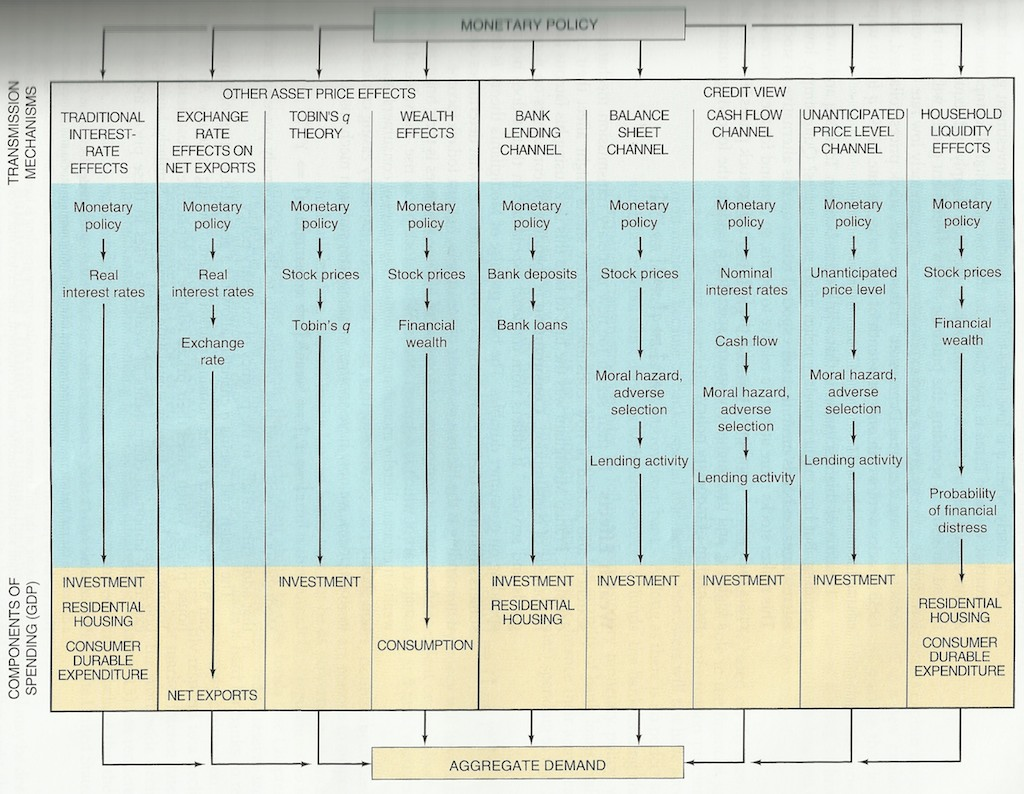
\includegraphics[scale=0.5]{./imgs/c26f1.jpg}
\end{center}

\end{document}
